\section{Initial Database Architecture}
\subsubsection*{Diagram ER}

\begin{figure}[H]
  \centering
  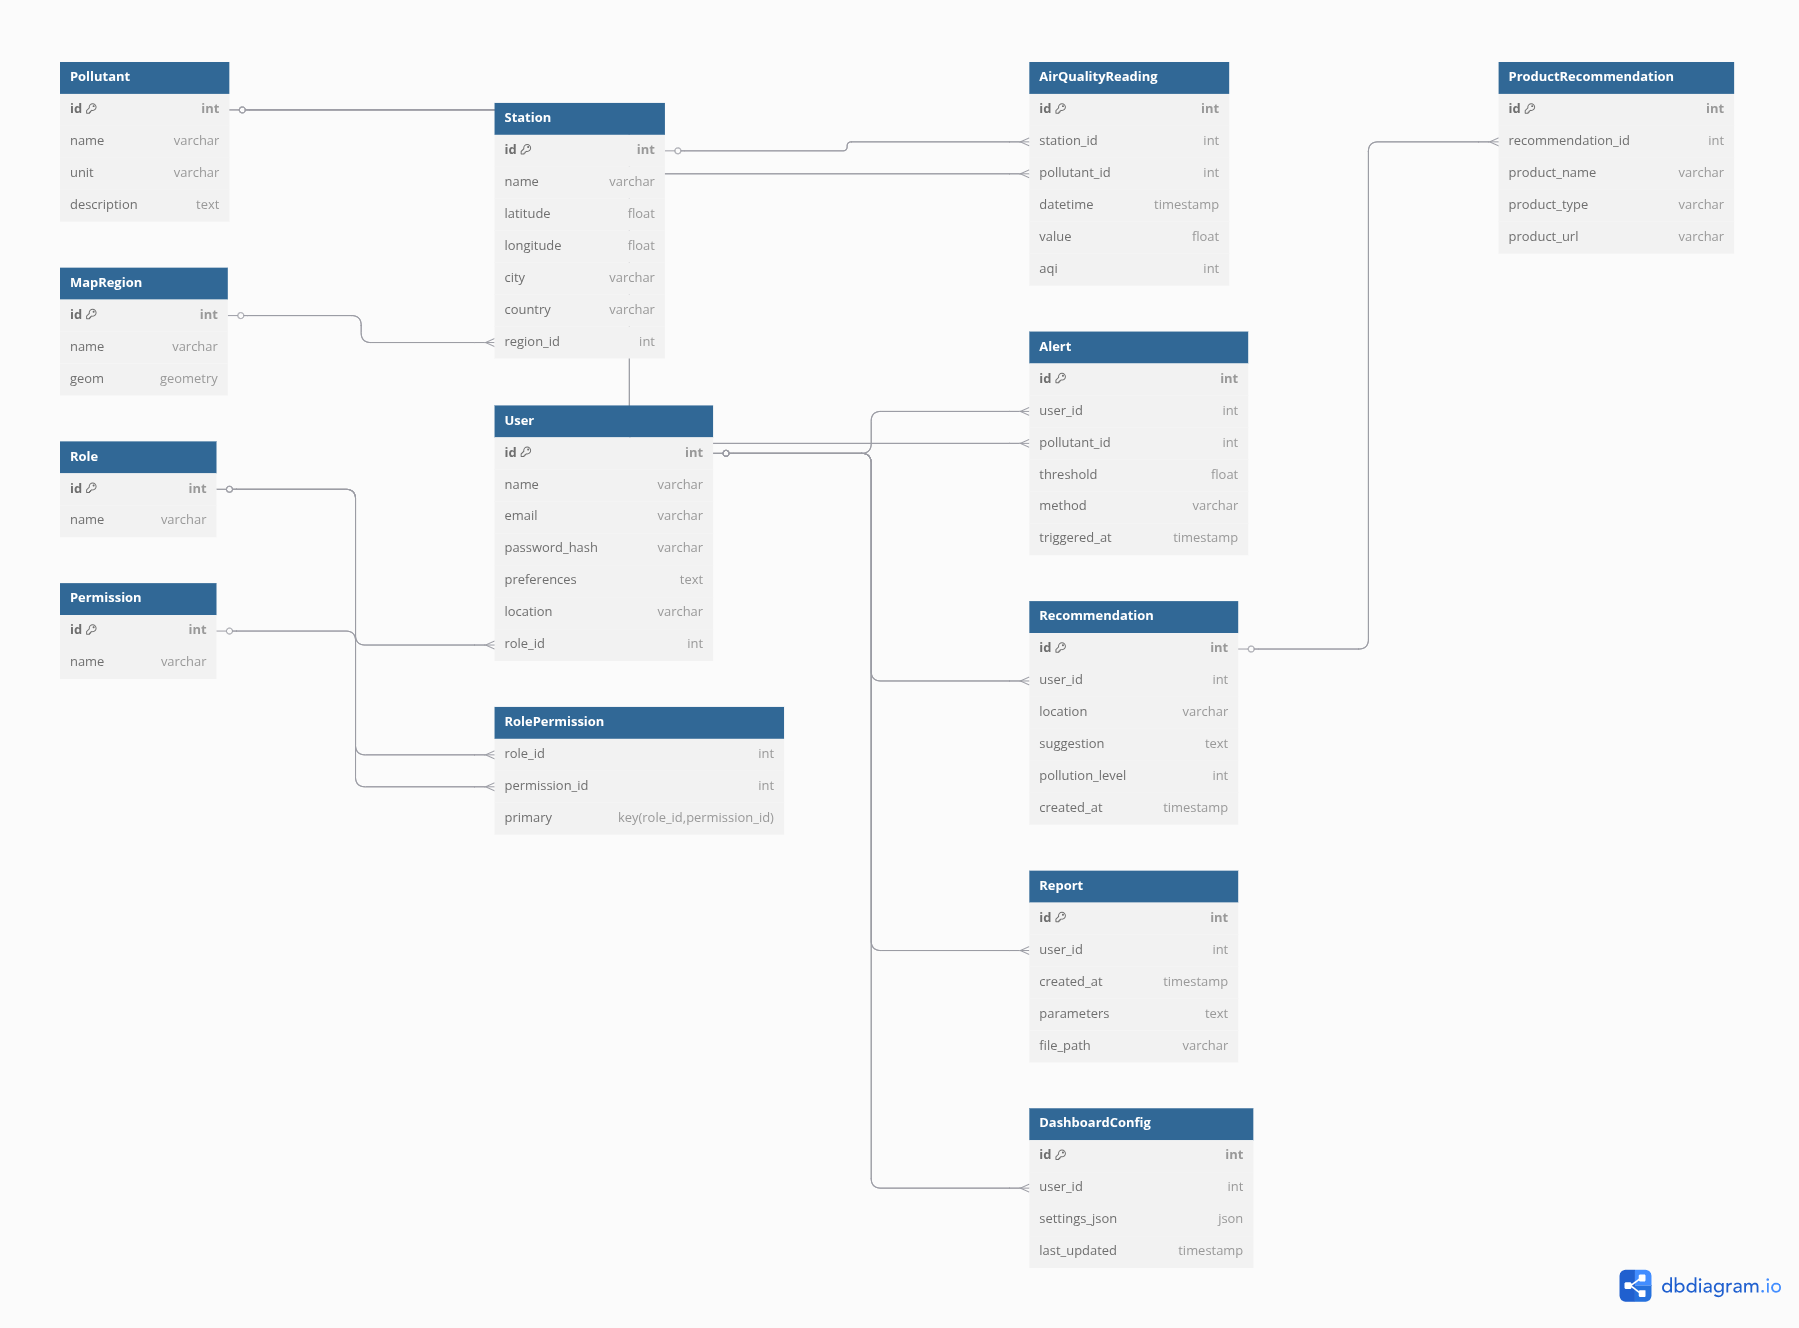
\includegraphics[width=\linewidth]{Imagenes/ER_Diagram.png}
  \caption{ER Diagram}
\end{figure}

\begin{longtable}{|p{3cm}|p{2cm}|p{6cm}|p{4cm}|}
\hline
\textbf{Component} & \textbf{Entity Name} & \textbf{Description} & \textbf{Attributes} \\
\hline
\endfirsthead

\hline
\textbf{Component} & \textbf{Entity Name} & \textbf{Description} & \textbf{Attributes} \\
\hline
\endhead

Geospatial Layer & Station & Monitoring station metadata and location. & id (PK), name, latitude, longitude, city, country \\
\hline

Geospatial Layer & AirQuality Reading & Air quality measurements from stations. & id (PK), station\_id (FK), datetime, pollutant\_type, value, aqi \\ 
\hline

Geospatial Layer & Pollutant & Catalog of pollutants and their units. & id (PK), name, unit, description \\ 
\hline

Customer Layer & User & Platform user and profile settings. & id (PK), name, email, password\_hash, preferences, location \\ 
\hline

Recommendation Engine & Alert & Alert configurations and triggered events. & id (PK), user\_id (FK), pollutant\_type, threshold, method, triggered\_at \\ 
\hline

Recommendation Engine & Recommen- dation & User-specific recommendations based on AQI. & id (PK), user\_id (FK), location, suggestion, pollution\_level, created\_at \\ 
\hline

Recommendation Engine & Report & Generated analytical reports. & id (PK), user\_id (FK), created\_at, parameters, file\_path \\ 
\hline

Geospatial Layer & MapRegion & Regions used for geospatial filtering and navigation. & id (PK), name, geom (geometry) \\ 
\hline

Customer Layer & Dashboard Config & User preferences for dashboard visualizations. & id (PK), user\_id (FK), settings\_json, last\_updated \\ 
\hline

Recommendation Engine & Product Recommen- dation & Suggested certified products during high pollution levels. & id (PK), recommendation\_id (FK), product\_name, product\_type, product\_url \\ 
\hline

Customer Layer & Role & Defines user roles in the platform (e.g., Admin, Citizen, Analyst). & id (PK), name (unique) \\ 
\hline

Customer Layer & Permission & Specifies distinct permissions that can be granted to roles. & id (PK), name (unique) \\
\hline

Customer Layer & Role Permission & Associates roles with permissions in a many-to-many relationship. & role\_id (FK), permission\_id (FK), PRIMARY KEY (role\_id, permission\_id) \\ 
\hline

\caption{Entities}
\end{longtable}